\documentclass[11pt]{article}

\newcommand{\specPdfTitle}{fsb: Design Specification}
\newcommand{\specHeader}{Design Specification}
% Shared by every specification in this folder. A document defines
% \specPdfTitle and \specHeader before inputting this file.
\usepackage[T1]{fontenc}
\usepackage[utf8]{inputenc}
\usepackage{lmodern}
\usepackage[margin=1in]{geometry}
\usepackage{microtype}
\usepackage{parskip}
\usepackage{amsmath}
\usepackage{amssymb}
\usepackage{amsthm}
\usepackage{mathtools}
\usepackage{booktabs}
\usepackage{longtable}
\usepackage{array}
\usepackage{enumitem}
\usepackage{needspace}
\usepackage{xcolor}
\usepackage{listings}
\usepackage{fancyhdr}
\usepackage{hyperref}
\usepackage{bookmark}
\usepackage{xurl}
\usepackage{tikz}
\usetikzlibrary{arrows.meta,positioning,fit}

\definecolor{codeblue}{HTML}{1F4E79}
\definecolor{codegreen}{HTML}{3A6B35}
\definecolor{codegray}{HTML}{555555}
\definecolor{codebackground}{HTML}{F5F7F9}
\definecolor{rulegray}{HTML}{D7DCE2}

\hypersetup{
  colorlinks=true,
  linkcolor=codeblue,
  urlcolor=codeblue,
  citecolor=codeblue,
  pdftitle={\specPdfTitle},
  pdfsubject={fsb, a read-only local file browser}
}

\lstdefinestyle{program}{
  basicstyle=\small\ttfamily,
  backgroundcolor=\color{codebackground},
  frame=single,
  rulecolor=\color{rulegray},
  framerule=0.4pt,
  xleftmargin=0.5em,
  xrightmargin=0.5em,
  aboveskip=0.8em,
  belowskip=0.8em,
  breaklines=true,
  columns=fullflexible,
  keepspaces=true,
  showstringspaces=false,
  keywordstyle=\color{codeblue}\bfseries,
  commentstyle=\color{codegreen},
  stringstyle=\color{codegray}
}

\lstset{style=program}

\newtheorem{law}{Law}[section]
\newtheorem{proposition}[law]{Proposition}
\theoremstyle{definition}
\newtheorem{definition}[law]{Definition}
\newtheorem{observation}[law]{Observation}
\newtheorem{boundary}[law]{Boundary}

\setlist{itemsep=0.25em, topsep=0.4em}
\setcounter{tocdepth}{2}
\setcounter{secnumdepth}{3}
\raggedbottom
\sloppy
\emergencystretch=3em

\pagestyle{fancy}
\fancyhf{}
\fancyhead[L]{\texttt{fsb}}
\fancyhead[R]{\specHeader}
\fancyfoot[C]{\thepage}
\setlength{\headheight}{14pt}


% Macros shared by every specification in this folder.
\newcommand{\code}[1]{\texttt{#1}}
\newcommand{\Tests}[1]{\par\smallskip\noindent\begingroup\raggedright\small\textit{Checked by:} \path{#1}\par\endgroup}

% A numbered requirement of the functional specification. The identifier is a
% label, so \rid{ID} is a link and a reference to an identifier that does not
% exist is reported by LaTeX as an undefined reference.
\newenvironment{req}[1]{\par\medskip\noindent\phantomsection\label{req:#1}\textbf{#1}\hspace{0.7em}\ignorespaces}{\par}
\newcommand{\rid}[1]{\hyperref[req:#1]{\textsf{#1}}}
% A requirement of the functional specification named from another document.
\newcommand{\fq}[1]{\textsf{#1}}
\newcommand{\shall}{\textit{shall}}


\title{\texttt{fsb}: Design Specification}
\author{}
\date{September 21, 2026 \\ Version 0.1 (draft)}

\begin{document}

\maketitle
\begin{abstract}
This document describes how \texttt{fsb} is built and why it was built that way:
its structure, the mechanism behind each guarantee in the functional specification,
the alternatives that were considered and rejected, how the design is tested, and
what it does not do.  It is written for people who maintain the program, review it, or
test it adversarially.  It changes when the construction changes; the functional
specification does not.  Requirement identifiers such as \fq{RUL-6} refer to the
functional specification.
\end{abstract}

\tableofcontents

\section{Principles}

The security of \texttt{fsb} rests on a few principles that the rest of the design
applies.  Each was, at some point, the lesson of a defect (Section~\ref{sec:history}).

\begin{description}
  \item[One chokepoint.]  Every read of the user's file system goes through one
        package, the \emph{guard}.  No package that serves HTTP may touch the file
        system, and a test fails the build if one imports \code{os}, \code{io/fs},
        \code{syscall} or \code{path/filepath}.  A property of the guard therefore
        holds for every endpoint at once.
  \item[Fail closed.]  When a decision cannot be made, the answer is refusal:
        a malformed rule file stops the program from starting; a file with several
        names is refused until its names are known; a path that cannot be resolved is
        not served.
  \item[Over-match to deny, decide by identity to allow.]  Comparing names can be
        wrong in either direction.  A deny check may safely match too much (it only
        blocks more); an allow check must not, and so decides by the identity of the
        file or folder (device and inode), never by the spelling of its name.
  \item[Name equality belongs to the volume.]  Whether two names are the same file is
        a fact about the file system, not about the program.  The program compares
        names the way the volume does, and tests that claim against the operating
        system rather than against its own model.
  \item[Decide from bytes, not names.]  What a file \emph{is} (an image, a PDF, an
        archive) is decided from its contents.  A name is at most a hint.
  \item[Read nothing that is not needed.]  Refusal is decided before any byte is
        read; a cloud-only file is never read implicitly, because reading it downloads
        it.
  \item[Each layer assumes the one before it failed.]  Rendered Markdown, for
        example, is escaped, then sanitized, then shown in a frame that cannot run
        anything of its own or reach the network.
  \item[Verify against the environment.]  The tests that matter most let the
        operating system decide the facts (Section~\ref{sec:verification}).
\end{description}

\subsection{Technology}

The back end is Go, using the standard library's HTTP server, with one extra
dependency for Unicode (\code{golang.org/x/text}, for normalization and case
folding) and one for extended attributes (\code{golang.org/x/sys}).  The front end
is Svelte 5 with TypeScript, built with Vite, and embedded in the binary with
\code{go:embed}; the compiled output is committed so that building the binary needs
no Node.  The front end has three runtime dependencies that ship in the output:
\code{marked} (Markdown), \code{dompurify} and \code{highlight.js}; Svelte is compiled away.
The result is a single binary of about 11~MB.

\section{Architecture}

\subsection{Components}

\begin{center}
\small
\begin{tabular}{@{}p{0.24\linewidth}p{0.66\linewidth}@{}}
\toprule
Component & Responsibility \\
\midrule
\code{cmd/fsb} & Command line, startup, the launch URL, opening the browser, shutdown; the remembered port, background mode and finding a running \texttt{fsb} (\code{config.go}, \code{background.go}, \code{process.go}). \\
\code{internal/rules} & The rule dialect: parsing, matching, name folding, the built-in rules. Knows nothing of files. \\
\code{internal/guard} & The chokepoint: opening, listing, searching, reading heads, metadata, sniffed endpoints, archive listing, the hard-link index. The only code that touches the file system on behalf of a request. \\
\code{internal/httpguard} & The middleware that makes a local web server safe: host and origin checks, the session, the prefix, security headers. Knows nothing of files. \\
\code{internal/quicklook} & Runs Apple's \code{qlmanage} to draw a Quick Look picture of a private copy that the guard made. The only code that runs another program on a file. Knows nothing of rules. \\
\code{internal/server} & The endpoints. Turns guard results into HTTP, and guard errors into status codes. \\
\code{web} & The embedded front end, and the fixed page that renders Markdown. \\
\code{e2e} & Browser tests, and their drivers for Chrome and Safari. \\
\code{specs} & These documents. \\
\bottomrule
\end{tabular}
\end{center}

\subsection{Structure}

\begin{center}
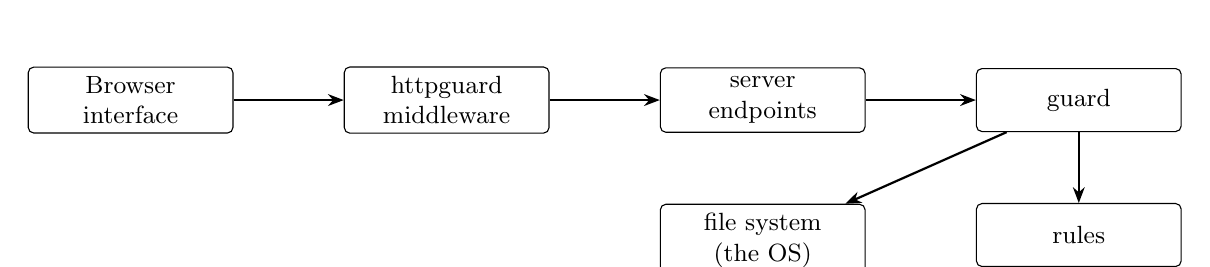
\begin{tikzpicture}[
  box/.style={draw, rounded corners=2pt, minimum width=2.6cm, minimum height=0.8cm, align=center, font=\small},
  arrow/.style={-{Stealth[length=2mm]}, thick},
  node distance=0.9cm and 1.4cm]
  \node[box] (browser) {Browser\\interface};
  \node[box, right=of browser] (hg) {httpguard\\middleware};
  \node[box, right=of hg] (srv) {server\\endpoints};
  \node[box, right=of srv] (guard) {guard};
  \node[box, below=of guard] (rules) {rules};
  \node[box, below=of srv] (fs) {file system\\(the OS)};
  \draw[arrow] (browser) -- (hg);
  \draw[arrow] (hg) -- (srv);
  \draw[arrow] (srv) -- (guard);
  \draw[arrow] (guard) -- (rules);
  \draw[arrow] (guard) -- (fs);
\end{tikzpicture}
\end{center}

Dependencies point one way: \code{server} uses \code{guard} and \code{httpguard};
\code{server} also uses \code{quicklook}, which draws only the copy that
\code{guard.CopyForQuickLook} made; \code{guard} uses \code{rules};
\code{rules}, \code{httpguard} and \code{quicklook} use nothing of the program's
own.  \code{cmd/fsb} assembles them.

\subsection{Life of a request}

\begin{enumerate}
  \item The HTTP server accepts the connection on the loopback address.
  \item The access log records the method, path and status, never the query
        (which is where the launch token travels).
  \item The middleware sets the security headers, then checks, in order: the
        \code{Host} header; the method; the \code{Origin}, \code{Referer} and
        \code{Sec-Fetch-Site} headers; that the path is under the random prefix
        (which it strips); the launch-token exchange; and the session cookie.  A
        failure of any check is the same 403 (\fq{SEC-2} to \fq{SEC-8}).
  \item The endpoint reads its parameters and calls one guard operation.
  \item The guard canonicalizes the path, checks it against the deny rules before and
        after opening, opens the file, verifies that what was opened is what was
        checked, and decides the file's kind from its bytes where needed.
  \item The endpoint turns the result into a response, and every guard error into a
        status code in one function (\code{fail}), so that denied, missing and
        outside-the-roots paths cannot be told apart by accident.
\end{enumerate}

\subsection{Startup}

\code{cmd/fsb} resolves the home folder to its real path.  \code{--init},
\code{--stop} and \code{--status} act and exit here, and \code{--background} starts
its child here (which runs these same steps from the start).  It then loads the two
rule files (or their built-in defaults); \code{--show-deny} and \code{--show-ignore}
print them and exit here, so they show exactly what would be enforced.  It then builds the guard from the roots (served once each, compared by
identity) and rules, names the credential locations the guard must also protect,
starts the hard-link index building in the background, binds the loopback port
(\code{choosePort}, Section~\ref{sec:port}), prints the launch URL, and only then
serves.  A failure at any step before serving stops the program with a message.

\subsection{The port, and background mode}
\label{sec:port}

Browsers keep local storage per origin, and the origin includes the port, so a port
chosen afresh at each start would reset every preference (\fq{CFG-4}).
\code{choosePort} therefore reuses the port in \code{\~{}/.config/fsb/lastport}, and
writes it after a start that did not use \code{--port} (best effort, like the front
end's own writes to local storage).  The random port was never a security control:
the boundary is the 256-bit launch token, the \code{Host} and \code{Origin} checks, and
the random path prefix, which still changes at every start.  \code{--port} is
deliberately not remembered, so that a one-off choice made to avoid a conflict heals
back to the usual port, and its preferences, once the conflict is gone.  If the
remembered port is taken, \code{fsb} fails rather than silently moving (which would
look as if it had lost the preferences); \code{portInUseMessage} asks \code{lsof} and
\code{ps} which program holds it so that the message can name it.

\code{--background} re-executes the program with \code{FSB\_BACKGROUND\_CHILD=1}
in a new session (\code{setsid}), so the child has no controlling terminal.  The
child's standard output and error are a writer (\code{handoff}) that goes to a pipe
on file descriptor~3 until the child is serving, then to
\code{\~{}/.config/fsb/background.log}.  The parent copies the pipe to its own output
until a fixed ready marker arrives (success: it releases the child and exits) or the
pipe closes without one (the child failed and has printed why; nothing is left
running).  The child records its process number in \code{\~{}/.config/fsb/pid} and
removes it on shutdown if it still names itself.

\code{findRunning} locates a running \code{fsb} for \code{--stop}, \code{--status} and
the refusal of a second \code{--background}: first the process in the PID file, then
the process listening on the remembered port.  Either is accepted only if \code{ps}
belongs to the same user and its executable file (from \code{/proc} or \code{lsof}, not
the name \code{ps} shows, which on macOS is the process's own \code{argv[0]}) is named
\code{fsb} or as the running binary is, and a process from the PID file must also have
the start time recorded there.  So a stale PID file whose number was reused, or another
program on the port that calls itself \code{fsb}, is never signaled.  \texttt{fsb}'s own
files are opened without following symbolic links and set to mode \code{0600}.

\section{The Guard}
\label{sec:guard}

\subsection{Opening a path}

Every operation begins by opening the path, in this order.  The order is the design.

\begin{enumerate}
  \item \textbf{Canonicalize.}  The path must be non-empty, contain no NUL, and be
        absolute.  It is cleaned lexically (\code{.}, \code{..} and repeated slashes
        removed) and reduced to one spelling of each alias (Section~\ref{sec:aliases}).
        URL-decoding has already happened, exactly once, in the HTTP layer; the guard
        never decodes, so a literal \code{\%2e\%2e} is just a name.
  \item \textbf{Lexical deny check.}  The cleaned path is matched against the deny
        rules \emph{before the file system is touched}.  The type of the final
        component is not yet known, so it is treated as a file here; a rule that
        applies only to folders is decided in step~7.  (Assuming a folder would refuse
        a plain file that shares its name with a \code{dir/} rule although listings
        show it.)
  \item \textbf{Open without blocking.}  The path is opened read-only and
        non-blocking, so that a pipe or a device cannot hang the server.  A permission
        error is examined (Section~\ref{sec:ancestor}) before it is reported.
  \item \textbf{Reject special files.}  On the descriptor, anything but a regular file
        or a folder is refused.  Only then is blocking restored.
  \item \textbf{Resolve and confirm.}  The real path is resolved (symbolic links
        followed), and the guard confirms that the file at that real path is the
        \emph{same file} as the open descriptor (device and inode).  If not, the path
        changed between the two steps and the request is refused as a race.
  \item \textbf{Roots and deny on the real location.}  The real path must lie inside a
        root (by identity, Section~\ref{sec:roots}), and must not match a deny rule.
  \item \textbf{Precise lexical check.}  With the type now known, the requested path is
        matched again.  A path is thus refused if \emph{either} its spelling or its real
        location is denied.
  \item \textbf{Other names.}  A regular file with several names is checked against
        the hard-link index (Section~\ref{sec:linkindex}).
\end{enumerate}

Everything that later reads bytes does so through the descriptor this returns, so
the decision and the read concern the same file.  Extended attributes, for example,
are read from that descriptor.

\subsection{Aliases}
\label{sec:aliases}

macOS keeps its user data on a separate volume whose folders appear at ordinary
paths through \emph{firmlinks}: \code{/Users} and \code{/System/Volumes/Data/Users}
are one directory.  Firmlinks are not symbolic links, so resolving links does not
reduce them, and a rule for \code{/Users/me/.ssh} would not match the longer
spelling.  Every path is therefore reduced to its ordinary form before any comparison
with a root or a rule.

The reduction compares path components one at a time, with the same name equality as
the rules (Section~\ref{sec:fold}), and rebuilds the path from the firmlink's own
spelling.  An earlier version sliced the path to the byte length of the prefix, which
cut a folded spelling (\code{/S}\emph{long-s}\code{ystem}) in the middle of a
character and left it unreduced.  The firmlink table is read from
\code{/usr/share/firmlinks}, with a built-in copy as fallback.

\subsection{Roots}
\label{sec:roots}

Each root is resolved to its real path at startup, and its identity (the file
information of the folder) is kept.  Whether a path lies inside a root is then decided
by taking the leading components of the path that correspond to the root and
comparing the \emph{identity} of that folder with the root's.  Comparing folded text
would be right on a case-insensitive volume but would admit a different sibling on a
case-sensitive one (\code{Public} for a root of \code{public}).  This is an allow
decision, so it must not over-match.

\subsection{Permission errors inside denied places}
\label{sec:ancestor}

An unreadable file inside a denied folder must look exactly like a missing one, or its
existence leaks.  When opening fails with a permission error, the guard resolves the
longest prefix of the path that can be resolved (an unsearchable folder stops the
resolution of what is inside it, not of the folder itself), rebuilds the full real
path from it, and applies the deny rules to that.  Only if nothing denies it is the
permission error reported.

\subsection{Listing}

A listing opens the folder as above and receives its real location.  Each child is
then judged by \emph{that} location and not by the symbolic link or alias the folder
was reached through, in one function used by both listing and search
(\code{entry}), so that search cannot show what listing would not.  For a child:

\begin{itemize}
  \item a symbolic link is resolved; a broken one is marked; one whose target is denied
        or outside the roots is omitted; the target's size, date and type are shown;
  \item the child's path is matched against the deny rules and, separately, the hide
        rules, each ignoring the ancestors above the folder itself (so entering a hidden
        folder on purpose shows its contents);
  \item a regular file with several names is checked against the hard-link index.
\end{itemize}

Entries are handed out in batches as the directory is read, which is what lets the
interface paint before a huge folder has been read.

\subsection{Search}

Search is a breadth-first walk, so shallow matches come first.  Every folder is opened
through the same operation, every child goes through \code{entry}, denied and hidden
folders are never entered, and symbolic links to folders are never followed (which
also rules out cycles).  It stops at a result limit or an entry limit and reports that a limit
stopped it.  Names are compared after the folding of Section~\ref{sec:fold}, or, for
\emph{Match case}, after normalization only.

\subsection{Cloud-only files}

On macOS a file that exists only in the cloud carries a flag in its file information.
The guard checks it before any read and reports the file as not downloaded; the head,
the metadata, the previews and the archive listing all refuse to read it.  Reading such
a file would make the system download it, which \texttt{fsb} must never do implicitly.
An explicit download by the user is the one path that reads it.

\subsection{Other files and endpoints}

\begin{description}
  \item[Head] reads at most a stated number of bytes from the descriptor, and returns
        text only if it is valid UTF-8 without control characters; binary contents never
        leave the guard.
  \item[Metadata] describes the entry, and reads extended attributes through the
        descriptor, capped in number and size.
  \item[Sniffed endpoints] (image, PDF, archive) share one routine that opens the file,
        reads its first bytes, decides the kind from them, and rewinds; they differ only
        in the test applied (Section~\ref{sec:content}).
\end{description}

\subsection{Hard links}
\label{sec:linkindex}

Rules name paths, and a hard link is another name for the same file, so a hard link to a
denied file is invisible to them.  The guard therefore judges a regular file with more
than one name by its identity: if any of its names is denied, all of them are.

\paragraph{The index.}  Finding the other names of a file means visiting every file
under the roots, because the operating system offers no way to ask.  A walk therefore
builds an index from identity to names, containing only regular files with more than one
name (a few dozen on a typical home folder), and the guard evaluates a file's names
against the deny rules.  The walk also covers the \emph{protected locations} named by the
program at startup (the credential folders of every home), so that a link from a served
folder to a credential file outside the roots is found.

\paragraph{The walk is in the background.}  On a home folder of 700{,}000 files it takes
about 18 seconds, which must not be spent inside a request.  It is started at startup.
While it has not finished, and for a file with several names that it has not seen (a link
made since), the file is \emph{refused}: guessing ``allowed'' would defeat the purpose.
A later walk that began after the file was first noticed and still does not find it
shows that the walker cannot see it, and the file is then allowed, so that nothing is
refused forever.  Walks are spaced by at least twice the time the last one took, and
bounded by an entry count and a time.

\paragraph{What is not covered.}  A denied name that lies outside every root and every
protected location, and links made after a walk was stopped by its limit, are not found.

\section{The Rule Matcher}
\label{sec:rulematcher}

\subsection{Matching}

A rule set is an ordered list of compiled rules.  For a path, the matcher evaluates
each prefix of the path in turn (the folder itself, its parent, and so on down to the
path), and the set \emph{excludes} the path if any prefix is excluded: an excluded
folder excludes everything in it, and no later rule (not even a negation) can bring it
back, as in git.  Within one prefix the last matching rule wins, which is what makes
negation in the ignore file work.  The deny file has no negation, so it is a plain
union of rules.

Matching a path \emph{below} a folder ignores the prefixes at or above that folder.  It is
used for the hide rules while listing, so that entering a hidden folder on purpose shows
what is inside it.

\subsection{Compiling a rule}

A rule is translated to a regular expression, case-insensitive and with the dot matching
a newline (so that a name containing a newline cannot defeat \code{**}), ending in
\code{\textbackslash s*\$}, so that a name with trailing white space still matches.  The
translation follows the gitignore glob: \code{*} and \code{?} do not cross a
separator; \code{**} matches folders; a class \code{[...]} never matches a separator
(a negated class excludes it explicitly, and a \code{/} inside a class is an error); a
trailing \code{/} makes the rule apply to folders only.  A pattern is anchored to the home
folder if it begins with \code{\~{}/}, is absolute if it begins with \code{/}, is relative
to the home folder if it contains a \code{/} elsewhere, and matches at any depth
otherwise or after a leading \code{**/}.

\subsection{Name equality}
\label{sec:fold}

Both the pattern and the path are folded before they are compared (\code{Fold}): Unicode
normalization (NFC), then \emph{full} case folding, then NFC again.  The rules must
match names as the volume compares them, and on macOS the case-insensitive volume uses
full folding, under which the sharp s equals \code{ss}, the long s equals \code{s},
the Kelvin sign equals \code{k}, and the ligatures \code{ff}, \code{fi}, \code{fl},
\code{ffi}, \code{ffl} and \code{st} equal their spelled-out forms.  Simple case
folding, which was used at first, treated these as different names, so
\code{\~{}/.\ss h} opened \code{\~{}/.ssh} while the rule for \code{.ssh} did not match.  The
set of aliases was \emph{measured} on the volume, by creating every one- and
two-letter name and probing every character in the Unicode range, and is a test.
The client-side filter uses the equivalent lower-, upper-, lower-casing, and the tests
check that the two agree on the measured aliases.

Names are compared this way so that a deny rule over-matches, which is safe.  Where the
result is an \emph{allow} (whether a path is inside a root), identity is used instead
(Section~\ref{sec:roots}).

\subsection{Speed}

Listing a folder evaluates the rules once per entry.  A rule set of about thirty rules
took about 29~$\mu$s per entry, which would add three seconds to a folder of 100{,}000
entries, so two optimizations were made, both of which must give the same answer as the
plain loop:

\begin{itemize}
  \item A rule whose pattern contains no slash can match only the last component of a
        path, so it is tested against that component alone (short and anchored) instead of
        against the whole path at every level.
  \item For a set without negation, all rules of each kind are combined into one
        expression, asked first; only when it says a match is possible are the rules
        consulted one by one, to say \emph{which} rule matched (for \code{--debug}).
\end{itemize}

The cost is about 9~$\mu$s per entry, and a property test checks that the quick path
never changes an answer.

\subsection{Loading a rule file}

A rule file is written by a person in an editor, and a deny rule that loads but never
matches is the worst outcome.  The parser therefore either normalizes or refuses.  It
strips a leading byte order mark (which otherwise broke the first rule) and accepts any
line ending (a bare carriage return joined lines).  It refuses, naming the line: an
inline comment, \code{\~{}name}, a quoted pattern, an invisible character, a lookalike
of the slash, negation in the deny file, and the malformed patterns of the
functional specification (\fq{RUL-12}).  Whatever loads, works as written.

\subsection{The built-in rules}

The core deny rules are compiled into the binary, so they apply even without a deny
file.  The credential rules are not anchored to the current home folder, because the same
folders exist in backups, clones, other accounts' homes and under a wrong \code{HOME}.  If
a deny file exists it is authoritative, and \code{CoreMissing} compares the core rules with the
file's rules \emph{as names} to decide which are not in effect.  The list of credential
locations for the hard-link index (Section~\ref{sec:linkindex}) mirrors the credential entries of
the core rules, for the given home and every folder in \code{/Users} and \code{/home}
(\code{homeParents}).  It names literal folders, so for Flatpak, whose rules match any
application ID, it names the usual IDs.  The list holds the locations of macOS and of
Linux on both systems (Section~\ref{sec:decisions}).

\section{The HTTP Layer}

\subsection{Middleware}

The middleware is a single function that either refuses a request or passes it on with
the prefix removed.  Its checks, and the order of them, are in the life of a request
(Section~\ref{sec:guard}); this section records the reasons.

\begin{description}
  \item[Host.]  A page on another name that resolves to the loopback address still
        sends its own name in the \code{Host} header, so an exact allowlist of the two
        loopback names with the port defeats DNS rebinding.  The port is fixed at start.
  \item[Origin, Referer, Fetch metadata.]  A browser serializes \code{Origin} as exactly
        scheme, host and port; anything else (a path, credentials, an opaque \code{null}) is
        refused rather than interpreted.  \code{Sec-Fetch-Site} must be \code{same-origin} or
        \code{none} (or absent, for clients that do not send it).  The value
        \code{same-site} is refused because a page on another port of the same host is
        same-site to the browser, so \code{SameSite=Strict} does not stop it.
  \item[Read-only.]  Only \code{GET} and \code{HEAD} reach a handler; the endpoint table
        contains no other method.
\end{description}

\subsection{The session and the prefix}

The launch token and the session value are 256-bit random values, compared in constant
time.  The token is exchanged once, atomically, for the session cookie, at the bare root
(\code{/?token=}); the response redirects to the prefixed root so the token leaves the
address bar and the history.  The launch URL does not name the prefix: it is handed to the
program that opens the browser, whose command line other users can read, and a user who
knew the prefix could have the user's browser send the cookie to a server of theirs on
another port (finding~47).

A cookie is scoped by host and by path, never by port.  A plain \code{Path=/} cookie would be
sent to every other web server on \code{127.0.0.1} that the same browser visits, and a server
that received it could replay it.  The design therefore serves everything under a random
128-bit path prefix chosen at start, sets the cookie's path to it, and refuses (403) any URL not
under it.  The browser then sends the cookie only for URLs under the prefix, which no other
server knows.  The prefix is a scope rather than a credential, since the session cookie is
still required; but it is kept from other users, because knowing it is what would let a
local server receive the cookie.  The
front end forms every URL relative to its own location so that this needs no configuration.

\subsection{The launch comes from the user's own connection (Linux)}
\label{sec:launchowner}

The launch URL is in the command line of the program that opens the browser (and on
Linux of the browser itself, until it first uses the URL), where other users can
read it.  On Linux, \code{exchange} therefore accepts a correct token only from a
connection whose client end belongs to \texttt{fsb}'s own user (\fq{SEC-16}).  The
order is the point: (1) a wrong token is refused with no lookup; (2) a token already
used is refused the same way, with no lookup and no warning, so replaying it costs
nothing and fills no log; (3) only then is the owner looked up, and a refusal leaves
the token unused, so another user who reads the URL and uses it first cannot keep
the user's own browser out; (4) the token is consumed atomically.  Refusals are
reported on standard error (\code{Config.Warn}), at most three times and once more
to say the rest are not, with the reason but never the token.

The lookup (\code{internal/connowner}) takes the server's and the client's address
from the request (\code{http.LocalAddrContextKey} and \code{RemoteAddr}, IPv4-mapped
addresses unmapped) and finds the row of \code{/proc/net/tcp} or \code{tcp6} whose
own address is the client's and whose peer is the server's: the client's end.
\texttt{fsb}'s own end lists the same two addresses the other way round, and would
name \texttt{fsb}'s own user, so matching it would let anyone through; the test
compares the matched row's socket inode with the client's.  Rows in ESTABLISHED,
FIN\_WAIT1 or FIN\_WAIT2 count (a client may close its sending side after its
request); TIME\_WAIT rows carry no owner.  The table's uid column is given in
\texttt{fsb}'s own user namespace, so a sandboxed browser (Flatpak, Snap) should show
as the user (not yet tried, Section~\ref{sec:untested}); the overflow uid, which every user the namespace cannot name shares, is
treated as unknown.  An unreadable table or a missing row is unknown too, and
unknown is refused: failing open would let the check be skipped by any condition
that hides a row.  A port forward counts as the user running it.

The same check applies to every request that carries a valid session cookie, so that a
cookie captured by another user, by whatever route, is refused.  It runs only after
the cookie is validated, so a request without the session costs no lookup, and its
result is remembered per connection (\code{httpguard.ConnContext}, installed as the
server's \code{ConnContext}): it is the owner that is remembered, not a verdict, and
only once found, so a lookup that fails is tried again on the next request rather
than refusing the whole connection; a browser's few kept-alive connections cost a few
lookups in all.  Refused launches and refused sessions have separate warning budgets.  macOS has no
comparable table, so there \code{RequireOwner} is given no lookup and both checks are
off.

\subsection{Headers and framing}

Every response carries the headers of \fq{SEC-9}.  Two endpoints relax framing, deliberately
and narrowly: the fixed Markdown page and the PDF may be framed by the interface's own pages
(\code{X-Frame-Options: SAMEORIGIN}, \code{frame-ancestors 'self'}), and the interface itself
may not.

\subsection{Streaming}

Listings and searches are newline-delimited JSON, flushed as batches are ready, because a
folder can hold hundreds of thousands of entries and the first screen must not wait for the
last.  A listing that breaks after it has begun ends with an error line rather than a status
code, since the status was already sent.  Pagination was rejected: the client sorts, and a
sort needs all entries, so streaming keeps the whole listing available and still paints early.

\subsection{Errors}

One function maps every guard error to a status.  Denied, outside-the-roots, nonexistent,
malformed and not-regular all map to the same 404 with the same body; only \code{--debug} adds
the rule name.  Permission errors on paths that passed every rule map to 403; cloud-only files to
409; wrong kinds to 415; anything unexpected to 500 with the detail in the log only.

\subsection{Streams end explicitly}

A listing and a search are streamed as newline-delimited JSON, and a response that simply
stops (a dropped connection, a server error after the header) would otherwise look like a
folder that was just short.  Both therefore end with a line that says how they ended: a
listing with \code{\{"done":true\}}, a search with \code{\{"done":true,\ldots\}} carrying
how many entries were visible, whether a limit stopped it, and whether part of it could
not be searched (\code{incomplete}); an error mid-stream is a line of its own instead.
The client requires the done line and treats a stream that ends without one as broken,
not as complete.

\subsection{Names on the wire}
\label{sec:wirenames}

A Linux name may be any bytes except \code{/} and NUL, so it need not be UTF-8, while
JSON strings are Unicode: Go's encoder replaces each byte that is not part of valid
UTF-8 with U+FFFD.  A file so named was listed under a name that does not exist, and
the client, which builds every request from the names it was given, could never ask
for it again.  \code{wireName} (\code{internal/server/wire.go}) therefore rewrites every
name and path the server puts in JSON (\fq{API-10}): valid UTF-8 is unchanged, and each
stray byte becomes NUL followed by two uppercase hexadecimal digits.  No name contains
NUL, so the result is never ambiguous, and \code{wireName} is one-to-one.  Copies are
rewritten (\code{wireEntries}, \code{wireMatches}, \code{wireMeta}); the guard's own
values are not touched, and the guard never sees an escape.  \code{wireArchive} also
passes archive members through it, but finds nothing to escape: the archive lister has
already replaced invalid UTF-8 in them (Section~\ref{sec:content}), since a member is
only ever displayed, never requested.

The return trip needs no decoder.  The client's \code{queryPath}
(\code{web/src/lib/format.ts}), the one place a path becomes a request, turns each
escape into the byte itself (\code{\%E9}) and percent-encodes everything else as UTF-8,
so the \code{path} parameter decodes, on the server, to the name's real bytes, which
the guard already handled.  Keeping the decoder out of the server keeps the escape out
of the security core: a request can only ever name real bytes.  On the screen,
\code{displayName} shows an escape as \code{\textlangle 0xE9\textrangle}, in the style
of the markers of \fq{NAM-2}; ``Copy path'' (\code{copyablePath}) writes the path in
the shell's \code{\$'\ldots'} quoting.  The address bar keeps the escaped form, which
\code{encodeURIComponent} carries as \code{\%00E9}.  A download's suggested name is
the name as received (\fq{NAM-2}), escape included; what a browser makes of a NUL in a
file name is its own choice, and has not been tested.

\subsection{Timeouts and shutdown}

The server sets a header-read timeout against slow clients and has no write timeout,
because streams may legitimately last.  On interrupt or termination it stops accepting requests and
gives requests in progress three seconds.

\section{Content-Typed Endpoints}
\label{sec:content}

Three endpoints look inside a file: inline images, inline PDFs, and archive listings.  Each is
defined by a test on the file's \emph{leading bytes}, never its name, and each opens the file
through the guard, so every property of Section~\ref{sec:guard} applies to it unchanged.  A
fourth, Quick Look pictures, is different in kind: macOS reads the document, not
\texttt{fsb} (Section~\ref{sec:quicklook}).

\subsection{Images}

An image is served inline only if its first bytes are a PNG, JPEG, GIF or WebP signature.
The response is sent with a policy that sandboxes it and allows no resources, so even a
crafted file has nothing to reach.  SVG is never accepted, because it can carry script, and
neither is HTML.  A file named \code{.png} that is not one is refused (415) and the interface
falls back to the ordinary file preview.

\subsection{PDFs}

A PDF is served inline only if it begins with \code{\%PDF-}.  It cannot be sent with the
\code{sandbox} policy that images get, because browsers then refuse to display it.  The
protection is instead the byte check, framing headers that allow only the interface's own
pages to embed it, a policy that forbids script in the response, and the browser's own PDF
viewer, which runs in an isolated component of its own.  The interface asks first, with a
one-byte range request, whether the file really is a PDF, and only then points a frame at it.

A viewer may take the keyboard focus by itself (Chrome's does, for an encrypted PDF's
password field), and once focus is inside the frame no key event reaches the interface.  The
preview pane records whether the pointer is over the frame and whether the last key was Tab;
when the window loses focus to the frame with neither, focus goes back to the list
(\fq{PRV-8}).

\subsection{Quick Look pictures}
\label{sec:quicklook}

For iWork and Office documents the preview is the PNG that Apple's \code{qlmanage -t}
draws, which is what Finder shows.  This is the one place \texttt{fsb} hands a file to
another program, and that program opens what it is given by itself, resolving more than the
guard can see: a Finder alias is a small regular file, marked by its \code{FinderInfo}
attribute, that Quick Look follows to its target.  An independent review showed that an
alias named \code{report.docx} made Quick Look draw a file in a denied folder, and one
outside the roots.  Quick Look is therefore never given the user's file.

\begin{enumerate}
  \item \textbf{A private copy.}  \code{guard.CopyForQuickLook} opens the document
        exactly as every endpoint does (roots, deny rules before and after, hard links to
        denied files), requires an iWork or Office extension on the real path, refuses a
        cloud-only document, and copies the bytes, from the descriptor it verified, into a
        fresh temporary folder that only the user can read.  A copy has no extended
        attributes and no resource fork, so an alias's copy is just its bytes, which Quick
        Look draws, at most, as a blank page; and nothing can be swapped between the check
        and the drawing.
  \item \textbf{Packages.}  A package document is walked without following links.  Every
        file in it is opened through the guard by its full path, and must still lie inside
        the package (a folder swapped for a link after the walk listed it leads elsewhere,
        and is caught here).  A part that is denied, a link, a hard link to a denied file or
        not a regular file is left out of the copy, as a listing leaves it out, so the
        answer does not reveal it (the same review found that refusing the whole package
        did); a cloud-only part refuses the package.
  \item \textbf{Bounds.}  A copy is limited to 256~MB and 5{,}000 entries.  Copying and
        drawing share two slots.  \code{qlmanage} never finishes on a document it cannot
        draw, so it runs under a 5-second deadline and is killed when the browser abandons
        the request.  Exactly one PNG under 20~MB must come out, or there is no picture.
        The picture is served like an image (sandbox policy, \code{nosniff}) and never
        cached, and the temporary folder is removed.
\end{enumerate}

Choosing by extension rather than by bytes (\fq{PRV-2}) is deliberate: Quick Look decides
what the document is, and a package is a folder with no bytes of its own.  The extension only
decides whether to ask.  Keynote's \code{.key} stays covered by the core rule \code{*.key}.

\subsection{Archives}

An archive listing returns names and sizes only, never member data, and nothing is extracted.
The format is decided from bytes: the zip signature, the \code{ustar} marker at offset 257 of a
tar, or a gzip stream that contains a tar.  The limits of \fq{LIM-1} bound a hostile file:

\begin{itemize}
  \item A zip's directory is held in memory by the standard library, so the guard first reads
        the end-of-central-directory record and refuses a zip that claims more entries than it
        will index (and, when the count is stored elsewhere in a very large zip, refuses by
        size).
  \item A tar is streamed, stopping at an entry limit; a gzip-compressed tar is read through a
        reader capped at a number of decompressed bytes, so a bomb costs a bounded amount of
        time and memory, and the listing says it was cut short.
  \item Member names are untrusted: control characters and invalid UTF-8 are replaced, and the
        interface additionally replaces bidirectional characters, and names are only ever
        displayed, never used as paths.
\end{itemize}

\subsection{Rendered Markdown}

Rendering a Markdown file must not run code, load anything remote, or reach the interface.
It is done in three layers, each assuming the one before failed.

\begin{enumerate}
  \item \textbf{Escaping.}  The Markdown is converted by a library configured so that raw HTML
        in the source becomes text; links carry no address at all (an attribute says what
        they mean: a file on the disk, or a web address); images carry no source (a marker names
        a local file); a remote or unsupported image becomes a text placeholder.  A link is
        resolved against the Markdown file's folder to a normalized absolute path, or dropped
        to plain text if it is not a relative path or an \code{http} or \code{https} address.
  \item \textbf{Sanitizing.}  The result goes through DOMPurify with a fixed list of allowed
        tags and attributes.
  \item \textbf{A sandboxed frame.}  The sanitized markup is sent by \code{postMessage} to a fixed
        page, framed with \code{sandbox="allow-scripts"} (so it has an opaque origin and no access
        to the session or the interface).  The page's own policy is \code{default-src 'none'}
        with images limited to \code{data:}, and admits its one script and one style
        \emph{by hash}, computed from the page at start so that a change to the page cannot
        silently invalidate the policy.  The page accepts messages only from its parent.
\end{enumerate}

Links are not followed inside the frame.  A click sends a message to the interface, which
validates it and either changes the location to the target file's folder with the file selected,
or opens a web address in a new tab without a referrer.  Images inside the roots are fetched by
the interface, through the guarded image endpoint, and passed in as \code{data:} URLs, because the
cookie's scope and \code{SameSite} would otherwise stop the opaque-origin frame from fetching them.
Opening a Markdown file therefore makes no request to anything outside the machine.

\section{The Front End}

\subsection{Structure}

The interface is a single page built with Svelte 5 (runes), TypeScript and Vite.  Its
logic is kept in small \emph{pure} modules, which import nothing from the browser, so that
they run under Node's own test runner: ordering (\code{sort}), filtering (\code{filter}),
column layout (\code{columns}), preferences (\code{prefs}), preview classification and text
helpers (\code{preview}), the path and location functions (\code{format}, \code{goto}),
the key mapping (\code{keys}), the Markdown conversion (\code{markdown}), and where the page was
loaded from (\code{base}).  The components hold only what needs the DOM.

\subsection{Decisions}

\begin{description}
  \item[Virtualized list.]  Only the rows on screen are drawn, from a scroll position and a
        fixed row height; a folder of 100{,}000 entries draws about 30 rows.
  \item[Location as state.]  The current folder, and the entry to select, are in the URL
        fragment (\code{\#/path?select=name}), which is never sent to the server, so folders
        are bookmarkable and Back works without any routing library.  Parsing is strict: a
        bad escape is not silently replaced.
  \item[Requests relative to the page.]  Every request is formed from the page's own
        directory, so the random prefix (which scopes the cookie) needs no configuration.
  \item[Sorting in the browser.]  The server streams entries in the order the file system
        gave them; the browser sorts, with a comparison that is a total order and does not
        depend on the input order (a test).  A time that cannot be parsed sorts as the oldest,
        so the order stays total.
  \item[Names are displayed, not trusted.]  Characters that would disguise a name are replaced by
        visible markers for display only.  Names are always inserted as text, never as markup.
  \item[Preferences are optional.]  They are kept in local storage with every read guarded, and
        every value falls back on its own.  Local storage is per origin, which includes the
        port; that is why the server remembers its port (Section~\ref{sec:port}).
  \item[The pane grows with the window.]  \code{clampPaneWidth} bounds the preview pane
        between 240 pixels and the window's width less \code{RESERVED\_FOR\_LIST}
        (320 pixels, matched by a CSS \code{max-width}), and the page tracks the window's
        width live, so the pane can widen with the window and is narrowed if the window
        shrinks.  An earlier fixed ceiling of 900 pixels was reported by the user as a
        usability limit, not found by a test.
  \item[Every letter types ahead.]  Search, Go to path and Copy are on Alt+S, Alt+G and
        Alt+C, read by physical key (\code{KeyboardEvent.code}) because macOS changes the
        character Option produces; so no plain letter is reserved and type-ahead
        (\fq{KEY-3}) can reach every name.
  \item[A click selects.]  A plain left click on a file name calls \code{preventDefault}, so
        it selects the row instead of following the link's \code{download} attribute;
        modified clicks and the context menu still reach the browser's own download
        (\fq{MOUSE-1}).
  \item[No dynamic code.]  There is no use of \code{eval}, of \code{innerHTML}, or of any
        other markup sink except one: the output of the syntax highlighter, which escapes its
        input.
\end{description}

\subsection{The preview pane as a state machine}

For a selected entry the pane is in one of a few states (idle, loading, folder, image, Quick
Look picture, PDF, archive, text, binary, empty, cloud-only, error).  A file name gives a \emph{hint}, the
server decides from the bytes, and a hint the server rejects falls back to the ordinary head
request, which never falls back again, so every run ends in a terminal state after at most two
requests.  (A Quick Look picture that fails falls back to that head request, or, for a package
document, which lists as a folder, straight to the folder state.)  Every request started for a selection, including a fall back, shares one
cancellation handle and is cancelled when the selection changes, so a late answer can never be
shown for the wrong file.  The laws are in the algebraic specification.

The Details panel (metadata and extended attributes) is a second, independent request
against the same selection, and keeps its own error state rather than sharing the main
preview's.  An earlier version used one shared variable for both: whichever request
settled last silently overwrote the other's message, and the panel's own error was
suppressed whenever the main preview had already failed, which could leave it reading
``Loading…'' forever even though its own request had already come back (Finding~18).

The folder listing has its own, separate error mapping (\code{describe} in
\code{App.svelte}), independent of the preview pane's, and it had never been given a case
for status 409: a cloud-only folder (Finding~19) fell through to the generic ``Server
error (\emph{n}).'' instead of the same cloud message the preview pane already shows for
a cloud-only \emph{file} (Finding~20).  Two error mappings for the same status code, one
of them incomplete, is the same shape of gap as Findings 4 through 6: a case a status code
can take that nothing had exercised.
Two independent outcomes need two independent variables.

\subsection{Hover peek}

A short delay before the request, a cache, a limit on simultaneous requests, and cancellation
on pointer movement, scroll or key press.  It requests the same head endpoint as the preview,
so it is subject to the same rules, and is off if the user turns it off.

\section{Verification}
\label{sec:verification}

The strategy follows the principles: the parts that decide what is served get the heaviest
testing, and the tests that matter most let the operating system decide the facts.

\subsection{Layers}

\begin{center}
\small
\begin{tabular}{@{}p{0.25\linewidth}p{0.65\linewidth}@{}}
\toprule
Layer & What it establishes \\
\midrule
Unit and integration (Go) & Behavior of the matcher, the guard, the middleware and every endpoint, including deliberately hostile paths. A test fails the build if an HTTP-facing package imports \code{os}, \code{io/fs}, \code{syscall} or \code{path/filepath}. \\
Property tests & The laws of the algebraic specification, with fixed seeds: monotonicity and order independence of deny, ancestor closure, fold invariance, listed implies openable, found implies listed, and the equivalence of the quick matching path with the plain one. \\
Fuzzing & The guard (with an oracle that does not trust \texttt{fsb}'s rules: whatever it returns must not be the same inode as a known secret or contain a secret marker), the matcher, the middleware, and the whole server stack. \\
Differential test against the OS & For each secret, thousands of generated spellings (case, folding aliases, decomposed accents, separators, dot segments, firmlink and symbolic-link aliases, named forks) are filtered by the operating system to those that really reach the secret, and every one must be refused. The reverse direction requires every such spelling of an ordinary file to be served. Reverting the folding fix makes it fail about 1{,}500 times. \\
Real-volume tests & Root containment on a real case-sensitive volume, run when a location for one is given. \\
Front-end tests (Node) & The pure modules, including the laws for ordering, filtering, location round trips, link resolution and name display. \\
Browser tests & A dependency-free suite written once against a driver interface, run with real keyboard and mouse events in Chrome (DevTools protocol) and Safari (WebDriver). It includes attacks from a second origin and from a page on another port, a DNS-rebinding hostname, the cookie's scope, and a 100{,}000-file folder. \\
Mutation checks & Removing a rule or reverting a fix must make a test fail; this was done for the folding fix, the cookie path, and others. \\
Algebra & The laws, and the defects found by stating them (Section~\ref{sec:history}). \\
\bottomrule
\end{tabular}
\end{center}

\subsection{Continuous integration}

On every change: formatting, vetting, the Go tests under the race detector, the front-end
tests, type checking, a build whose output must equal the committed one, an audit of the
packages that ship, the Chrome browser tests, and timed fuzzing of the four fuzz targets.
A scan for known vulnerabilities in the Go modules runs as well.  The Go tests run on macOS
and Linux; the rest on Linux.  The workflow runs on GitHub's hosted runners for every push to
a private repository; its first run (2026-10-02) found finding~28 of
Section~\ref{sec:history}, and every run since has passed.

\subsection{What testing does not establish}

None of this is a guarantee.  It is a record of what was checked.  A fuzzer reaches only what
its fixture contains, and an early version missed a bug for that reason; the differential test
exists because reasoning about names had been wrong.  Findings~17 through~20
(Section~\ref{sec:history}) were caught by none of the automated layers: no fixture
anywhere contained a UNIX domain socket or a real File Provider placeholder folder, so
nothing had ever exercised the errno either produces, and the Details-panel race needed a
preview that fails, which no test happened to select.  All four were found by using the
running application, not by any automated layer, which is itself a reason to keep doing
that rather than treating the test suite as the last word; Finding~21 was found while
fixing them, by reading the surrounding code rather than by any test.  An independent
review was done three times, by an assistant (Section~\ref{sec:untested}), the second and
third finding defects in the fixes of the one before (Section~\ref{sec:history}); a
professional penetration test was not done.

\section{Decisions and Alternatives}

Each row is a decision that shaped the design, with what else was possible and why it was not
chosen.

\begin{center}
\small
\begin{longtable}{@{}p{0.20\linewidth}p{0.20\linewidth}p{0.52\linewidth}@{}}
\toprule
Decision & Rejected & Why \\
\midrule
\endhead
Write from scratch in Go with an embedded Svelte front end & Fork an existing multi-user file manager & The existing one is built around a jailed root, configuration in its own UI, and create, rename and delete. The security model here (whole home, read only, two-tier rules) is different in kind, and a fork would carry code paths that must not exist. \\
Two tiers: hide and deny & One list & Hiding clutter is cosmetic and must not be a security control; blocking must be absolute, not overridable, and load only from the global file so that a folder cannot relax it. Deny wins over ignore. \\
Deny loads only from the global file & Per-folder deny files & A per-folder file could be planted in the tree being browsed to weaken protection. \\
Core rules built in and active by default & Ship them commented out, with a warning & A tool that exposes \code{\~{}/.ssh} until configured is unsafe by default. The warning now covers only the case where the user weakened them. \\
Bind loopback only, not configurable & A flag for other interfaces & There is no safe way to serve the whole home folder to a network, so the option is not offered. \\
Single-use launch token, then a cookie & A permanent token in the URL & A token left in history or a shell must be useless. \\
Path prefix scoping the cookie & A plain cookie; a custom header on every request & Browsers cannot scope cookies by port. A header cannot accompany images, frames, PDFs and downloads. A random path scopes the cookie exactly. \\
Identity for hard links, from a background index & A hash of contents; a synchronous walk & A hash flags harmless copies, reads every candidate, and answers a different question. A synchronous walk did not finish in four seconds on a real home folder and would stall a request. Refusing until known keeps it safe meanwhile. \\
Roots decided by identity & Comparing folded text & Right on a case-insensitive volume, wrong on a case-sensitive one. \\
Full case folding, from \code{x/text}, applied to rules & \code{ToLower} & The volume uses full folding; simple folding made some spellings of a denied name invisible to the rules. \\
Refuse a file whose kind the bytes do not confirm & Trust extensions & An extension is chosen by whoever named the file. \\
Markdown in a sandboxed frame, sanitized, with a hash-pinned policy & Render in the page with a sanitizer only & One layer failing must not compromise the session; the frame has no origin, no network and one fixed script. \\
PDF in the browser's viewer in a frame with narrow framing headers & Bundle a PDF library; sandbox the frame & A library is large and a second parser to defend; a sandboxed frame is refused by browsers. \\
Stream listings as newline-delimited JSON & Pagination & The client sorts, which needs all entries; streaming paints early and keeps them all. \\
Sort in the browser & Sort on the server & The sort key and options change often; the total-order comparison is a pure, testable function. \\
Pure modules tested with Node's runner & A browser test for every function & Fast, dependency-free, and the laws are stated on them. \\
Commit the compiled front end & Build it in the Go build & Building the binary must need no Node. CI checks that the committed output is current. \\
Deny checks over-match; allow checks decide by identity & One equality for both & The two directions fail differently: over-matching a deny only blocks more, over-matching an allow serves the wrong folder. \\
Refuse files with several names until the index is ready & Allow until known & The window in which a hard link to a secret is served must be zero, at the cost of a short unavailability. \\
Hand-written manual page in roff & Generate it from Markdown & No build dependency, and the format users expect. \\
\bottomrule
\end{longtable}
\end{center}

\section{Limitations, Risks and History}
\label{sec:history}

\subsection{Risks}

\begin{description}
  \item[R1: sensitive paths are exposed by default.]  The root is the home folder, so without
        protection \code{\~{}/.ssh} and similar would be reachable.  Mitigated by the core deny
        rules, active by default and built in, and by a startup notice and a banner if the user
        weakens them.  Residual: a secret with an unremarkable name outside the core list, the optional
        rules left off, and a user who disables the core rules and ignores the warning.
  \item[R2: files with several names.]  Path rules cannot see a second name for a file.  Covered
        for denied names under the roots and for the credential locations, by refusing any file whose
        names are not all accounted for; see the limits below.
  \item[R3: untrusted content in a page that holds a session.]  Markdown, PDF and archive names are
        rendered or shown; mitigated by the layers of Section~\ref{sec:content}.
  \item[R5: another program reads the user's documents.]  Quick Look draws iWork and Office
        documents with Apple's generators.  Mitigated by giving it only a private copy of what the
        guard would serve, with bounds on size and time; residual: a flaw in a generator, as when
        Finder shows the same picture.
  \item[R4: permission prompts.]  macOS asks permission the first time for Documents, Desktop,
        Downloads and external volumes; the documentation says so.
\end{description}

\subsection{Known limitations}

\begin{itemize}
  \item A denied name outside every root and every protected credential location is not found as another
        name of a file, so a file with such a name is refused (a pnpm store outside the root, or a
        clone made with \code{git clone --local}, can make ordinary files unavailable).  A listing or a
        search may show a name or a size up to one second after the file was renamed onto a denied name;
        opening the file never does.  Cancellation of copying and listing is cooperative: a read that the
        file system is itself holding up cannot be interrupted, and keeps a Quick Look slot until it
        returns.  Search completeness does not include cloud-only folders, which are skipped on purpose.
  \item Response timing is not equalized: a denied path can be answered slightly faster than a missing
        one.  The status and body are identical.
  \item Anything that runs as the user can read the same files.  \texttt{fsb} is not a sandbox against
        local malware.
  \item The metadata endpoint reads a symbolic link's text from the requested path after the file was
        opened; an attacker who could rewrite that link during the call could learn the text of a denied
        path (not its contents).  Requires a same-user attacker.
  \item Rule files are read at startup only.
  \item On macOS the launch URL is visible to other users for the moment \code{open} runs, and
        no connection-owner check exists there.  On Linux, a port forward the user runs counts as
        the user, and where the owner of a connection cannot be determined (no \code{/proc}, WSL,
        some sandboxes) the launch URL is refused, so \texttt{fsb} cannot be used there.
  \item \code{--stop} would take another program of the same user for \texttt{fsb} if that
        program's executable file were itself named \code{fsb}.
  \item Under emulation (an amd64 container on Apple silicon), \code{--status} and \code{--stop}
        cannot recognize \texttt{fsb}: QEMU makes every emulated process's \code{/proc/PID/exe}
        name itself.
  \item Not yet tried with real cloud-placeholder files or in Firefox; a real mouse drag of a column
        header in Safari is unverified.
  \item The browser test for Safari occasionally fails in a run of tests that need a focused window,
        and passes on rerun.
\end{itemize}

\subsection{History of defects found by the design's own checks}

Stating the laws of the algebraic specification, auditing every comparison of names and paths,
and using the running application, and running it on Linux, found forty-eight defects, all fixed and each covered by a test where
the underlying condition could be reproduced at all (Section~\ref{sec:untested} says where it could not).
In brief:

\begin{enumerate}
  \item Simple case folding let \code{.\ss h} open \code{.ssh} (a bypass of a deny rule).
  \item A plain file named like a folder-only rule was listed but could not be opened.
  \item A negated glob class could match across a path separator.
  \item A row order that was not transitive when a time could not be parsed.
  \item The filter and the search disagreed about the sharp s.
  \item A stale fallback request could show the wrong file's preview.
  \item Firmlink prefixes were matched by byte length (a bypass under a root of \code{/}).
  \item Root containment compared spellings (wrong on a case-sensitive volume).
  \item Breadcrumbs, selection and the core-rule warning compared names by spelling.
  \item The credential rules were anchored to one home folder.
  \item A hard link to a credential file was served.
  \item The session cookie followed the host, not the port.
  \item A hard link to any other denied file was served.
  \item Rule files that loaded without error and did nothing.
  \item Secrets under other names (\code{id\_rsa}, certificate stores, password databases).
  \item File names that disguised themselves with bidirectional characters.
  \item Opening a UNIX domain socket used an errno (\code{EOPNOTSUPP}, or \code{ENXIO} on
        Linux) that the guard's error map did not recognize, so it surfaced as an opaque
        500 instead of the same ``not found'' every other special file gets.  Found from a
        screenshot of the running application, not from any test.
  \item The preview pane's Details panel shared one error variable with the main preview
        and hid its own message whenever the main preview had already failed, so it could
        read ``Loading…'' forever even though its own request had already finished.  Found
        alongside the previous defect, in the same screenshot.
  \item Listing or searching a folder that is itself a cloud-only placeholder (a File
        Provider domain such as OneDrive or iCloud Drive can make a whole folder dataless,
        not only the files in it) went straight into reading its directory entries, which
        the provider's virtual file system answered with something the guard's error map
        did not recognize, surfacing as an internal error instead of the same cloud
        message a dataless \emph{file} already gets.  Found from a screenshot of a real
        OneDrive folder, not from any test: no fixture anywhere had a real cloud-only
        placeholder, only a synthetic flag on individual files.
  \item The folder listing's own error mapping, separate from the preview pane's, had no
        case for status 409, so once the previous defect was fixed at the guard level the
        interface still showed ``Server error (409).'' for a cloud-only folder instead of
        explaining it.  Found alongside the previous defect.
  \item While fixing the above, a latent defect in \code{Search}: a directory reopened
        from its queue that turned out no longer to be a directory (a rare race) left its
        descriptor open, because the code path that skipped it predates the fix and never
        closed what \code{Open} had just handed it.  The new dataless check would have
        turned this from a rare race into a routine leak, since a cloud-only subfolder
        hits the same code path on every walk that reaches one.
  \item Found by the user: a root given twice (\code{--root \~{}} when the home folder is
        already the default root) was served twice, and the interface, which keys its list of
        roots by path, failed so that every folder looked empty.  Roots are now served once,
        compared by identity.
  \item Found by the user: Chrome's PDF viewer moves the focus to the password field of an
        encrypted PDF, after which no key reached the interface, so arrowing through a folder
        stopped dead on that file.  Focus now returns to the list unless the user clicked or
        tabbed into the viewer.
  \item Found by the second independent review (and confirmed): a Finder alias named like an
        Office document made Quick Look draw the alias's target, which could be denied or outside
        the roots.  Quick Look now draws a private copy (Section~\ref{sec:quicklook}).
  \item Found by the same review: refusing a package document that held a denied part answered
        differently from a clean package, revealing what a listing hides.  Such parts are now
        left out of the copy.
  \item Found by the same review: \code{--stop} took any process whose \code{argv[0]} ended in
        \code{fsb} for \texttt{fsb}.  It now checks the owner, the executable file and the
        recorded start time (Section~\ref{sec:port}).
  \item Found by the same review: \texttt{fsb}'s own files in \code{\~{}/.config/fsb} were
        written through symbolic links.  They are now opened without following links.
  \item Found by the first run of continuous integration: the module named Go 1.26.0, whose
        standard library has since had security fixes (reported by \code{govulncheck}); the
        developer's machine happened to use a newer release.  The module now names the
        toolchain (Go 1.27.1).  The same run found two tests that assumed macOS.
  \item Found by an external review (October 2026, eleven findings, all confirmed and fixed;
        the commits cite them by number).  The ones that mattered most: a file with several names that
        the index had not seen was \emph{allowed} during the rebuild cooldown (the code returned the
        wrong flag, and the tests, which set the cooldown to zero, hid it); the index trusted names
        recorded at the last walk; a zip's entry limit compared a 16-bit count with 200{,}000, so it
        could never trip, and the standard library built the whole directory first; the index walk and
        the Quick Look package copy entered cloud-only folders; a symbolic link to \code{/} passed a
        check that only looked at spellings; an image fetch read its whole body before checking its
        size; search's work limit ignored entries it excluded; a tar.gz stopped exactly at a member
        boundary looked complete; an old search's timer overwrote a new search's results; resize-handle
        keys also moved the selection; and a collator that compares digits by value left
        \code{file1} and \code{file01} in an order that depended on the input.
  \item Found by an independent review of those fixes: two more hard-link bypasses and a quadratic
        cost in the index, and zips written to a pipe were refused.  Fixing them with a change-time test
        was itself broken by the next review (renaming a folder renames its files without touching
        them), which led to the policy of Section~\ref{sec:linkindex}: serve a file only when every name
        is accounted for, now.  A third round refined it (names folded by parent identity; one
        retry walk).
  \item Found by a second review of the whole (seven findings, all medium): a hard-link verdict
        remembered for the length of a listing or search hid a rename that kept the link count; a
        folder queued for search could be swapped for a symbolic link before it was entered; the
        one retry walk a short-counted file is owed was spent by a lookup during the cooldown that
        could not start it; the wrapper that added cancellation hid \code{Seek}, so listing a plain
        tar read every member's body; a copy that ran out of time while a read was blocked reported
        success when the read returned end of file; a folder that could not be opened left a search
        looking complete; and an empty extended attribute that grew between two system calls was
        sliced out of an empty buffer and panicked.  A third review confirmed each fix and found
        nothing new.  Two choices came out of it and are stated as limits rather than hidden: the
        one-second reuse of a verdict, and cooperative (not hard) cancellation.
  \item Found by the Linux distribution tests (October 2026; fixed in 1.0.2): the core rules
        named only the macOS locations of browser data, so on Linux the Chrome, Chromium and
        Firefox profiles, the GNOME and KDE keyrings and the \code{pass} store were served; and
        the identity protection of credential folders looked for other homes only in
        \code{/Users}, not \code{/home}.
  \item Found while fixing the previous one: Brave and Edge were protected on neither system
        (1.0.2); and, once the Linux rules were in, Flatpak keeps an application's settings in
        \code{\~{}/.var/app/ID/config}, which they did not reach (1.0.4).
  \item Found by the same tests: \code{--status}, \code{--stop} and the port-holder message ran
        \code{ps} and \code{lsof}, which minimal Debian, Fedora and Arch lack and BusyBox's
        \code{ps} cannot serve, so \code{--stop} said no \texttt{fsb} was running while one
        served; and a running \texttt{fsb} whose file had been replaced, as by a rebuild, was not
        recognized, because Linux appends \code{" (deleted)"} to \code{/proc/PID/exe}.  Linux now
        reads \code{/proc} (1.0.3).
  \item Found by the same tests: a name that is not UTF-8 reached the client as U+FFFD, under a
        name that does not exist, and could not be opened (1.0.3,
        Section~\ref{sec:wirenames}).
  \item Found by probing Quick Look on Linux: with no Quick Look, \texttt{fsb} still copied the
        document and then ran any program called \code{qlmanage} on \code{PATH} (1.0.5).
  \item Found by an independent review of findings 32 to 36 (October 2026; 1.0.6): the
        Linux rules still missed Snap Chromium (\code{\~{}/snap/chromium/common/chromium}),
        although this document and the README said the rules covered Snap; Firefox 147's new
        profile location (\code{\~{}/.config/mozilla}); Flatpak apps' own keyrings; and, on
        macOS, Chromium and Chrome Beta and Canary.  Vivaldi, Opera, Thunderbird and the NSS
        key store were added with them.
  \item Found by the same review: the PID file recorded the start time as local-time text, so
        \code{--stop} under another \code{TZ} did not find a background \texttt{fsb} and
        removed its PID file (on macOS since 1.0).  The record is now independent of the time
        zone (Section~\ref{sec:port}).  The same review found that one half of the test of
        \code{--stop}'s impostor check was refused by the start-time check before it reached
        the impostor check, and that the preview pane's Copy path skipped the shell quoting
        of finding 35.
  \item Found by the vulnerability scan of continuous integration on 2026-10-09: six advisories against the
        standard library's \code{net/http} in Go 1.27.1 (GO-2026-6603, -6609, -6611, -6612,
        -6613, -6617).  Four concern the HTTP/2 server, which \texttt{fsb} never uses; the
        unbounded \code{Range} header was reachable through downloads with a session.  Fixed by
        Go 1.27.2 (1.0.7).
  \item Found by installing 1.0.7 the way a user does: \code{go install} ignores a module's
        \code{toolchain} line, so the pinned Go 1.27.2 reached no one who installed a release, and
        every earlier release had been built with whatever Go the user had.  The module's
        minimum (\code{go} line) is now 1.27.2, which an older Go downloads (1.0.8).
  \item Found by an independent review of opening the browser on Linux (1.0.9): the background
        child passed its handoff pipe and its marker variable to the browser it started, so a
        browser holding the pipe kept \code{fsb --background} waiting, and an \texttt{fsb} later
        started from the browser's process tree took itself for a background child, printing
        nothing and taking over the PID file (Section~\ref{sec:port}).
  \item Found by the same review: without a display, \code{xdg-open} ran \code{w3m}, which fetched
        the launch URL itself and left the printed one used up, with no message.
        \code{xdg-open} is no longer run without a display.
  \item Found by the same review: the launch URL, in the command line of \code{xdg-open} and the
        browser, could be read by another user, who could use it first and take the session.
        First documented (1.0.9), then closed on Linux by accepting the launch only from a
        connection of \texttt{fsb}'s own user (Section~\ref{sec:launchowner}, 1.0.10).
  \item Found by the same review: Control-C and \code{fsb --stop} waited out the opener's grace
        period, and a background instance stopped during it was reported as running.
  \item Found by an independent review of the launch-owner check: after the user's browser had
        used the token, another user could present it without limit, each time making
        \texttt{fsb} read the connection table and print a warning (about 4\,GB of log an hour).
        A used token is now refused before any lookup, and warnings are limited.
  \item Found by the same review: the check took the overflow uid, which every user an unusual
        user namespace cannot name shares, for an owner; missed a client that closes its sending
        side after its request; reported an unreadable table as a missing row; and, with
        \texttt{fsb} run as root, blamed ``another user'' for the user's own browser.  The tests
        compared owners by uid only, so a lookup that matched \texttt{fsb}'s own end of the
        connection, letting anyone through, would have passed them; they now compare socket
        inodes.
  \item Found by an independent review of the whole core before the final release
        (reproduced with Chromium and two users): the launch URL named the path prefix,
        and since 1.0.9 it was in a command line other users can read.  A server of another
        user on another port, asked by a page the user's browser visited once for a URL
        under the prefix, received the session cookie and could replay it.  The launch URL
        now names no prefix, and on Linux a request with the cookie must come from the
        user's own connection (Section~\ref{sec:launchowner}, 1.0.11).
  \item Found by the same review: under \code{--root /}, \code{/.nofollow/}\emph{path}
        named a file a second time and kept the prefix through symbolic-link resolution,
        so a deny rule anchored to a place did not match it (Section~\ref{sec:aliases},
        1.0.11).  The differential test had tried every alias but only against secrets that
        rules matching a name anywhere protect.
\end{enumerate}

The lesson common to several: name equality is a property of the volume, so deny checks may over-match but
allow checks must decide by identity.  Findings 17, 18, 19 and 20 are a different lesson: an error path that
no test happened to reach (no fixture had ever contained a real socket, a real cloud-only folder, or a
selected file whose main preview fails) is still worth trying by hand.  Findings 29 to 31 are a fourth: a fix can introduce the next defect (a wrapper that hid
\code{Seek}, a retry spent before it ran, a memo that outlived the facts it summarized), so each
fix got a test that fails without it, and the reviews were repeated until one found nothing.  Finding 24 is a third: handing a
path to another program hands over that program's idea of what the path means, which the guard cannot
check; the safe input is bytes the guard has already read.  Findings 32 to 36 are a fifth: a test suite that
passes on a platform is not use of the program there.  The Go tests had run on Linux in continuous
integration since the first day, yet each of these appeared only when \texttt{fsb} was run on Linux
distributions, as a user would; the same work found that two tests had never tested what they
claimed there (the extended-attribute test skipped on the containers' file system, and the test of
\code{--stop}'s impostor check used \code{sleep} and \code{nc}, which on BusyBox exit at once when
started under another name).  Findings 37 and 38 add a sixth: a claim in the
documentation is as much in need of review as the code; ``covers Snap'' had been written,
and read, without anyone listing which Snap packages keep which folder.  Findings 39 to 48
add a seventh: what reaches the user is the release as installed, and the programs
\texttt{fsb} starts.  Every check had passed inside the repository, where the
\code{toolchain} line applies; only installing the tag as a user would showed that it
did not.  A program \texttt{fsb} starts inherits more than its arguments (descriptors,
environment, a terminal), and is itself a channel another user can read.

\subsection{Milestones}

\begin{center}
\small
\begin{tabular}{@{}p{0.16\linewidth}p{0.36\linewidth}p{0.36\linewidth}@{}}
\toprule
Milestone & Scope & Status \\
\midrule
M0 Skeleton & Repository, CI, guard, matcher, middleware & Done. \\
M1 Crawl & Browsing, listing, filtering, sorting, rules & Done; 100{,}000-file folder measured. Daily use by the author still to confirm. \\
M2 Walk & Preview, hover peek, search, attributes, columns, rendered Markdown, PDF, archives & Built and tested in Chrome and Safari; not yet on real cloud placeholders or in Firefox. \\
Hardening & The audits and defects of the preceding subsection & Done, including independent reviews in October 2026 of 1.0 (three rounds, the last finding nothing new), of the Linux work, of opening the browser on Linux, of the launch-owner check, and of the whole core before the final release, and continuous integration on macOS and Linux.  A professional penetration test was planned but, by the owner's decision, not done. \\
M3 Public release & Public repository, documentation, a source release & Done: version 1.0 (October 2026), source only; no binaries and no Homebrew formula, by decision. \\
Linux check & Five distributions in Docker; \code{/proc}, \code{/sys}, \code{/dev}; extended attributes; Quick Look; the browser suites against four distributions; an independent review & Done, October 2026: findings 32 to 38, fixed in 1.0.2 to 1.0.6. \\
Linux browser & Opening the browser with \code{xdg-open}; the launch only from the user's own connection; Go 1.27.2 & Done, October 2026: findings 39 to 48, fixed in 1.0.7 to 1.0.11. \\
M4 Run & The stage-three requirements of the functional specification & Not planned: the project is finished and provided as-is. \\
\bottomrule
\end{tabular}
\end{center}


\end{document}
